\begin{figure}[H]
    \centering
    \begin{tikzpicture}[scale=1.0]
        \coordinate (a) at (-2.8,0);
        \coordinate (x) at (0,0);
        \coordinate (b) at (2.8,0);

        % Reta real.
        \draw[->, thick] (-3.6,0) -- (3.6,0) node[right] {$\mathbb R$};

        % Intervalo aberto.
        \draw[Cerulean!80!black, very thick] (a) -- (b);
        \filldraw[fill=white, draw=Cerulean!80!black, thick] (a) circle (2.6pt);
        \filldraw[fill=white, draw=Cerulean!80!black, thick] (b) circle (2.6pt);
        \filldraw[black] (x) circle (2pt);

        % Marcadores dos pontos principais.
        \draw[dotted] (a) -- ++(0,0.55);
        \draw[dotted] (x) -- ++(0,0.85);
        \draw[dotted] (b) -- ++(0,0.55);

        \node[below] at (a) {$a=x-r$};
        \node[below] at (x) {$x=\dfrac{a+b}{2}$};
        \node[below] at (b) {$b=x+r$};

        % Escolha do raio.
        \draw[Red, thick, <->] (-2.8,0.58) -- (0,0.58)
            node[midway, above] {$r=\dfrac{b-a}{2}$};
        \draw[Red, thick, <->] (0,0.58) -- (2.8,0.58)
            node[midway, above] {$r$};
    \end{tikzpicture}
    \caption{$]a,b[=B(x,r)$.}
\end{figure}
